
\documentclass[12pt]{beamer}
\usepackage[serbian]{babel}
\usepackage{mathrsfs}
\usepackage{amssymb}
\usepackage{amsmath}
\usepackage{amsthm}
\usetheme{default}
\usepackage{enumitem}
\usepackage{textcomp}
\usepackage{color}
\usepackage{url}
\usepackage{graphicx}
\usepackage{mathtools}
\definecolor{zelena}{rgb}{0.0, 0.5, 0.0}
\definecolor{plava}{rgb}{0.137,0.466,0.741}
\usepackage{listings}
\usepackage{xcolor} % for setting colors

% set the default code style
\lstset{language=C++,
     xleftmargin=20pt,
      basicstyle=\ttfamily,
      morekeywords={to, downto, then},
      keywordstyle=\color{blue}\ttfamily,
      stringstyle=\color{red}\ttfamily,
      commentstyle=\color{green}\ttfamily,
      morecomment=[l][\color{magenta}]{\#},
}

\lstset{escapeinside={@}{@}}

\usepackage{pgf,tikz}
\usetikzlibrary{arrows}
\usetheme{default}
\setbeamercolor{structure}{fg=beamer@blendedblue}
\definecolor{beamer@blendedblue}{rgb}{0.137,0.466,0.741}
\usecolortheme{whale}
\usefonttheme{professionalfonts}

\usepackage{ragged2e}
\addtobeamertemplate{block begin}{}{\justifying}

\newtheorem{thm}{Teorema}[section]
\theoremstyle{definition}
\newtheorem{dfn}{Definicija}[section]
\theoremstyle{remark}
\newtheorem{pr}{Problem}[section]
\theoremstyle{plain}
\newtheorem{lem}[thm]{Lema}
\date{3. maj 2018}

\usepackage{multicol}

\title{Pluton}
\author{Jelena Mrdak \\ Neboj\v sa Koturovi\' c} 

\begin{document}


\begin{frame} 
\titlepage
\end{frame}

% \usebackgroundtemplate{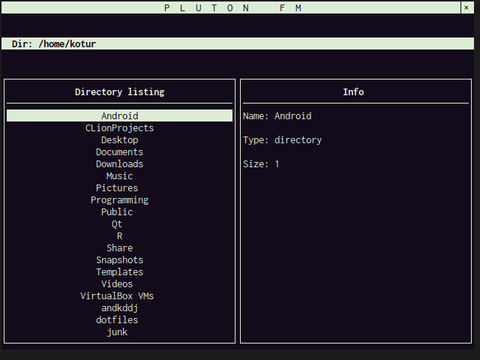
\includegraphics[width=\paperwidth,height=\paperheight]{img/1.png}}
\begin{frame}{Pluton}
  \begin{figure}[H]
    \centering
    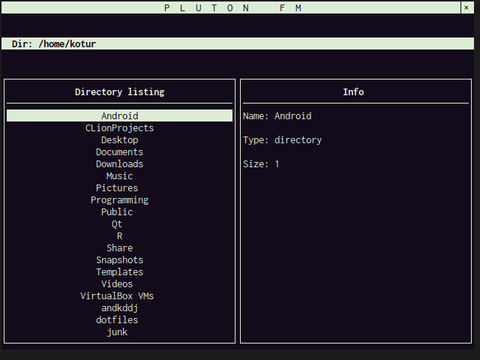
\includegraphics[width=5cm]{img/1.png}
  \end{figure}
  \begin{itemize}
    \item File manager 
    \item Jezik: C++
    \item Standard: c++17
    \item Biblioteke: Immer, CPPurses, FS Experimental
  \end{itemize}
\end{frame}
\usebackgroundtemplate{}


\begin{frame}[fragile]{Paradigma}
\lstset{language=C++,
    basicstyle=\tiny
}
  \begin{lstlisting}[mathescape=true]
class Current_dir {
private:
  fs::path path;
  immer::flex_vector<File> dirs;
  immer::flex_vector<File> regular_files;

public:
  Current_dir(const std::string& path, 
    immer::flex_vector<File> dirs, immer::flex_vector<File> regular_files);
  Current_dir(const std::string& path);
  immer::flex_vector<File> ls() const;
  Current_dir cd(const File& dir) const;
  Current_dir cd(fs::path dir_path) const;
  Current_dir rename(const File& f, const std::string& new_file_name) const &;
  Current_dir insert_file(File&& f) const &;
  Current_dir delete_file(const File& f) const &;
  const File find_by_fname(const std::string &file_name) const;
  const File& get_by_index(unsigned i) const;
  int get_index_by_name(const std::string &file_name) const;
};
  \end{lstlisting}
\end{frame}

\begin{frame}[fragile]{Immer}
immer je biblioteka imutabilnih struktura podataka napisana u C++
  \begin{lstlisting}[mathescape=true]
  immer::vector<int> v = {1,2,3}; 
  immer::vector<int> w = v.push_back(4); 
  print(v); // 1, 2, 3
  print(w); // 1, 2, 3, 4
  \end{lstlisting}
\end{frame}

\begin{frame}{Komande}
\begin{tabular}{c | c}
  taster & akcija\\
  \hline
  j & selektovanje narednog fajla \\
  k & selektovanje prethodnog fajla \\
  l/Enter & ula\v zenje u selektovani direktorijum\\
  h/Backspace & ula\v zenje u roditeljski direktorijum\\
  q & insertovanje novog regularnog fajla\\
  w & insertovanje praznog direktorijuma\\
  e & poretanje programa nad selektovanim fajlom\\
  r & preimenovanje selektovanog fajla\\
  u & undo \\
  p & redo \\
  Esc & Exit
\end{tabular}
\end{frame}
\end{document}

